%-------------------------------------------------------------------------------

% This file is part of Code_Saturne, a general-purpose CFD tool.
%
% Copyright (C) 1998-2013 EDF S.A.
%
% This program is free software; you can redistribute it and/or modify it under
% the terms of the GNU General Public License as published by the Free Software
% Foundation; either version 2 of the License, or (at your option) any later
% version.
%
% This program is distributed in the hope that it will be useful, but WITHOUT
% ANY WARRANTY; without even the implied warranty of MERCHANTABILITY or FITNESS
% FOR A PARTICULAR PURPOSE.  See the GNU General Public License for more
% details.
%
% You should have received a copy of the GNU General Public License along with
% this program; if not, write to the Free Software Foundation, Inc., 51 Franklin
% Street, Fifth Floor, Boston, MA 02110-1301, USA.

%-------------------------------------------------------------------------------

\programme{bilsc2}

\vspace{1cm}
%%%%%%%%%%%%%%%%%%%%%%%%%%%%%%%%%%
%%%%%%%%%%%%%%%%%%%%%%%%%%%%%%%%%%
\section*{Function}
%%%%%%%%%%%%%%%%%%%%%%%%%%%%%%%%%%
%%%%%%%%%%%%%%%%%%%%%%%%%%%%%%%%%%

In this subroutine, called by \texttt{codits} and \texttt{turbke}, the
contributions to the explicit budget of the reconstructed (on
non-orthogonal meshes and if the user chooses to) convective and
diffusive terms of the right-hand side of a convection/diffusion
equation for a scalar $a$ are computed. These terms
write \footnote{They appear on the right-hand side of the incremental
system for cell $I$ of the momentum prediction step:
$\mathcal{EM}(\delta\vect{u}^{k+1},I) =
\mathcal{E}(\vect{u}^{n+1/2,k},I)$  (see \fort{navstv} for more details)}:

\begin{equation}\label{Base_Bilsc2_eq_continue}
\begin{array}{ll}
\mathcal{B_{\mathcal{\beta}}}((\rho\,\vect{u})^{n},a)
&=\underbrace{-\dive(\,(\rho \vect{u})^{n}a)}_{\text {convective part}}
+\underbrace{\dive(\,\beta\,\grad a)}_{\text{diffusive part}}\\
\end{array}
\end{equation}

with $\rho$, $\vect{u}$, $\beta$ and $a$ the variables at time  ${t^n}$.

%%%%%%%%%%%%%%%%%%%%%%%%%%%%%%%%%%
%%%%%%%%%%%%%%%%%%%%%%%%%%%%%%%%%%
\section*{Discretization}
%%%%%%%%%%%%%%%%%%%%%%%%%%%%%%%%%%
%%%%%%%%%%%%%%%%%%%%%%%%%%%%%%%%%%
\subsection*{\bf Convective Part}
Using the notations adopted in the subroutine \fort{navstv}, the
explicit budget corresponding to the integration over a cell
$\Omega_i$ of the convective part $-{\dive(\,(\rho\,\vect{u})^n a)}$
of $\mathcal{B_{\mathcal{\beta}}}$ can be written as a sum of the
numerical fluxes $F_{\,ij}$ calculated at the faces of the internal
cells, and the numerical fluxes $F_{\,b_{ik}}$ calculated at the
boundary faces of the computational domain $\Omega$. Let's take
$\Neigh{i}$ the set of the centres of the neighbouring cells of
${\Omega_i}$ and $\gamma_b(i)$ the set of the centres of the boundary
faces of ${\Omega_i}$ (if they exist). Thus we can write

\begin{equation}\notag
\int_{\Omega_i}{\dive( (\rho \vect{u})^n  a )\, d\Omega} =
\sum_{j\in \Neigh{i}}{F_{\,ij}((\rho \vect{u})^n, a)}
+\sum_{k\in {\gamma_b(i)}} {F_{\,{b}_{ik}}((\rho \vect{u})^n,a)}
\end{equation}

with :
\begin{equation}
F_{\,ij}((\rho \vect{u})^n,a) = \left[{(\rho \vect{u})_{\,ij}^n} \text{.}\, \vect{S}_{\,ij}\right]\ a_{\,f,ij}
\end{equation}

\begin{equation}
F_{\,{b}_{ik}}((\rho \vect{u})^n, a) =  \left[{(\rho \vect{u})_{\,{b}_{ik}}^n} \text{.}\, \vect{S}_{\,{b}_{ik}}\right]\ {a_f}_{\,{b}_{ik}}
\end{equation}
where $a_{\,f,ij}$ and ${a_f}_{\,{b}_{ik}}$ represent the values of
$a$ at the internal and boundary faces of ${\Omega_i}$, respectively.\\

Before presenting the different convection schemes available in \CS, we define:\\
\begin{figure}[h]
\hspace*{1cm}\parbox{8cm}{%
\centerline{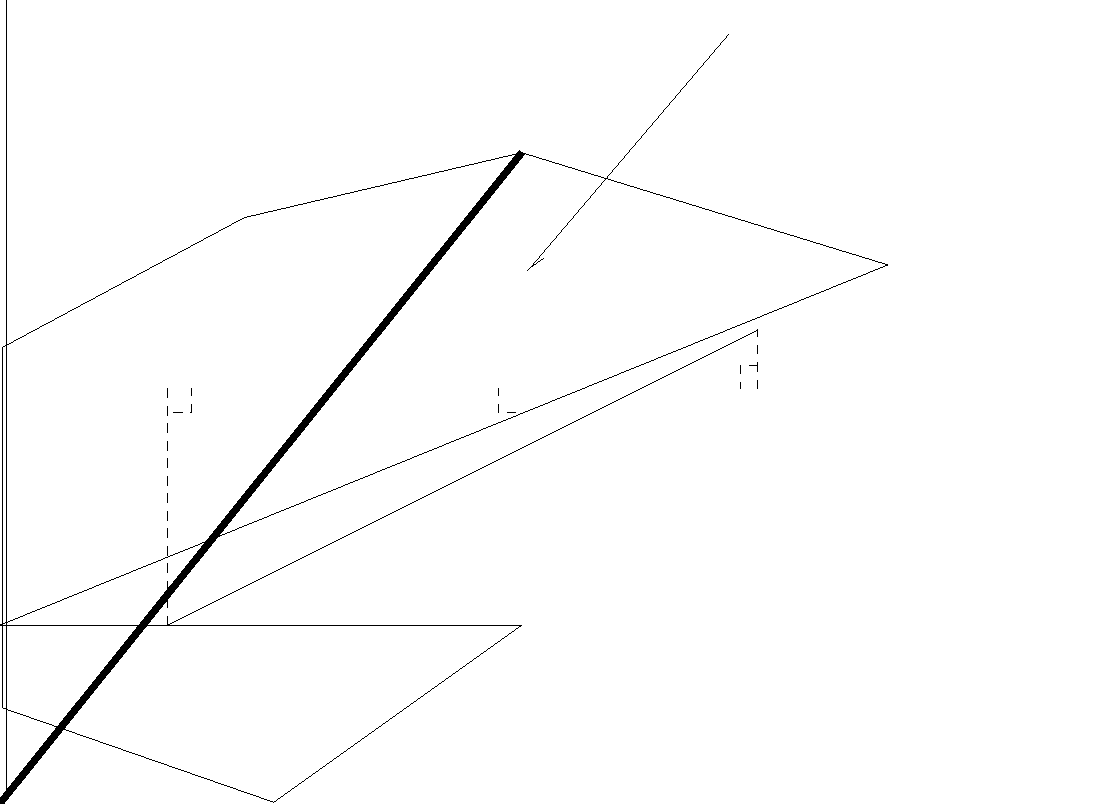
\includegraphics[height=4cm]{facette}}}
\parbox{8cm}{%
\centerline{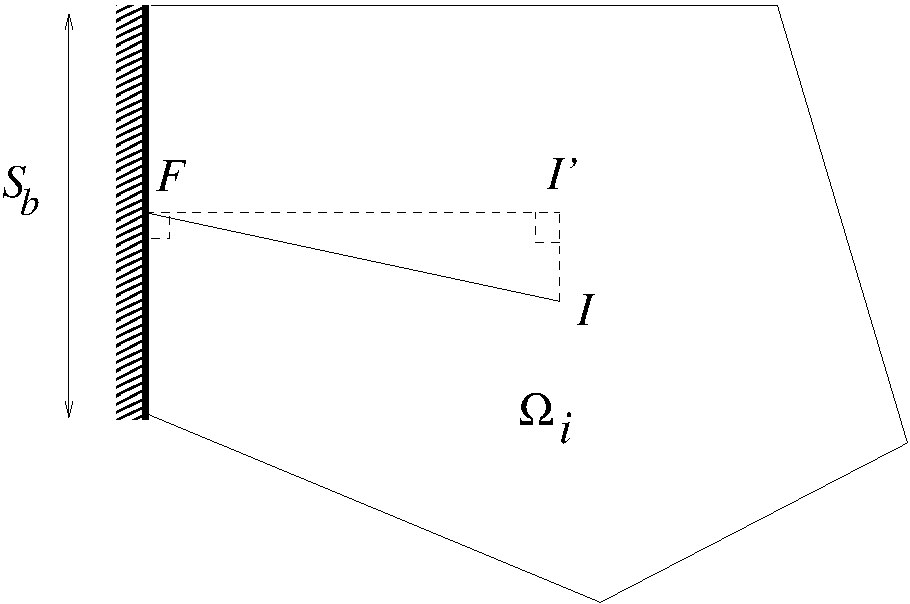
\includegraphics[height=4cm]{facebord}}}
\caption{\label{Base_Bilsc2_fig_geom}Definition of the geometric entities for internal (left) and a boundary faces (right).}
\end{figure}
\begin{equation}\notag
\displaystyle\alpha_{ij}=\frac{\overline{FJ'}}{\overline{I'J'}} \text{\ defined at the internal faces only and}
\end{equation}
\begin{equation}\notag
\vect{u}_{K'} = \vect{u}_{K}+(\ggrad{\vect{u}})_K\text{.}\, \vect{KK'}\, \text{\ at the first order in space, for ${K = I \,\text{or}\, J}$}
\end{equation}\\
The value of the convective flux ${F_{\,ij}}$ depends on the numerical scheme. Three different types of convection schemes are available in this subroutine:


\renewcommand{\arraystretch}{2.}
\begin{tabular}{ll}
\multicolumn{2}{l}{$\bullet\ $a $1^{st}$ order upwind scheme:}\\
&$F_{\,ij}((\rho \vect{u})^n,a)=
F^{\it{ upstream}}_{\,ij}((\rho \vect{u})^n,a)$\\
o\`u :&
$a_{\,f,ij}= \left\lbrace\begin{array}{l}
a_I \text{ si }(\rho \vect{u})_{\,ij}^n\,.\,\vect{S}_{\,ij}\geqslant 0\\
a_J \text{ si }(\rho \vect{u})_{\,ij}^n\,.\,\vect{S}_{\,ij} < 0
\end{array}\right.$\\

\multicolumn{2}{l}{$\bullet\ $a centered scheme:}\\
&$F_{\,ij}((\rho \vect{u})^n,a)=
F^{\text{\it{ centered}}}_{\,ij}((\rho \vect{u})^n,a)$\\
with :&$a_{\,f,ij}= \alpha_{ij} a_{I'}+(1-\alpha_{ij}) a_{J'}$\\
\multicolumn{2}{l}{$\bullet\ $a Second Order Linear Upwind scheme (SOLU):}\\
&$F_{\,ij}((\rho \vect{u})^n,a)=
F^{\text{\it { SOLU}}}_{\,ij}((\rho \vect{u})^n,a)$ \\
with :&
$a_{\,f,ij}=\left\lbrace\begin{array}{l}
a_I +\vect{IF}\,.\,(\grad a)_{\,I}
\text{\ \  si }(\rho \vect{u})_{\,ij}^n.\ \vect{S}_{\,ij}\geqslant 0\\
a_J + \vect{JF}\,.\,(\grad a)_{\,J}
\text{\ \  si }(\rho \vect{u})_{\,ij}^n.\ \vect{S}_{\,ij} < 0
\end{array}\right.$\\
\end{tabular}\\
\renewcommand{\arraystretch}{1.}
\footnotetext{Extrapolation  of the upwind value at the faces centre.}

The value of $F_{\,b_{ik}}$ is calculated as :
\begin{equation}\notag
{a_f}_{\,{b}_{ik}}=\left\lbrace\begin{array}{l}
a_I \text{ \ \ \ \ if }(\rho \vect{u})_{\,{b}_{ik}}^n
\text{.}\, \vect{S}_{\,{b}_{ik}}\geqslant 0\\
a_{\,{b}_{ik}}\text{ \ \ if } (\rho \vect{u})_{\,{b}_{ik}}^n
\text{.}\, \vect{S}_{\,{b}_{ik}} < 0
\end{array}\right.
\end{equation}
$a_{\,{b}_{ik}}$ is the boundary value directly computed from the prescribed boundary conditions.

\minititre{Remark 1}

When a centered scheme is used, we actually write (to ensure first order discretization in space for $a$) 

\begin{equation}\notag
a_{\,f,ij} = \alpha_{ij} a_I +  (1-\alpha_{ij}) a_J  + \displaystyle
\frac{1}{2}\left[(\grad a)_I+(\grad a)_J\right] \text{.}\, \vect{OF}
\end{equation}

A factor $\displaystyle \frac{1}{2}$ is used for numerical stability reasons.

\minititre{Remark 2}
A slope test (which may introduce non-linearities in the convection operator) allows to switch from 
the centered or SOLU scheme to the first order upwind scheme (without blending). Additionally, in standard mode $a_{\,f,ij}$ is computed as a weighted average between the upstream value and the centered value (blending), according to users' choice (variable $\var{BLENCV}$ in the subroutine  \fort{usini1}).


\subsection*{\bf Diffusive Part}

Similarly, the diffusive part writes :

\begin{equation}\notag
\int_{\Omega_i}{\dive(\,\beta\ \grad a)\  d\Omega} =
\sum_{j\in \Neigh{i}}{D_{\,ij}(\,\beta, a)}
+\sum_{k\in {\gamma_b(i)}} {D_{\,{b}_{ik}}(\beta, a)}
\end{equation}
with:
\begin{equation}
D_{\,ij}(\,\beta, a) = \beta_{\,ij}
\frac{a_{\,J'}- a_{\,I'}}{\overline{I'J'}} S_{\,ij}
\end{equation}
and :
\begin{equation}
D_{\,b_{ik}}(\,\beta, a) = \beta_{\,b_{ik}}
\frac{a_{\,b_{ik}}-a_{\,I'}}{\overline{I'F}} S_{\,b_{ik}}
\end{equation}
using the same notations as before, and with $S_{\,ij}$ and $S_{\,b_{ik}}$ being the norms of  vectors 
$\vect{S}_{\,ij}$, and $\vect{S}_{\,b_{ik}}$ respectively.

%%%%%%%%%%%%%%%%%%%%%%%%%%%%%%%%%%
%%%%%%%%%%%%%%%%%%%%%%%%%%%%%%%%%%
\section*{Implementation}
%%%%%%%%%%%%%%%%%%%%%%%%%%%%%%%%%%
%%%%%%%%%%%%%%%%%%%%%%%%%%%%%%%%%%

In the following, the reader is reminded of the role of the variables used in the different tests:
$\bullet \ $ \var{IRCFLP}, from array \var{IRCFLU} ; indicates for the considered variables wether 
or not the convective and diffusive fluxes are reconstructed \\ 
\hspace*{1cm}$ = 0$ : no reconstruction\\
\hspace*{1cm}$ = 1$ : reconstruction\\
$\bullet \ $ \var{ICONVP}, from array \var{ICONV} ; indicates if the considered variables is convected or not.\\
\hspace*{1cm}$ = 0$ : no convection\\
\hspace*{1cm}$ = 1$ : convection\\
$\bullet \ $ \var{IDIFFP}, from array \var{IDIFF} ; indicates if the diffusion of the considered variables is 
taken into account or not.\\
\hspace*{1cm}$ = 0$ : no diffusion\\
\hspace*{1cm}$ = 1$ : diffusion\\
 $\bullet \ $ \var{IUPWIN} indicates locally, in \fort{bilsc2} (to avoid unnecessary calculations) whether a pure upwind scheme is chosen  or not for the considered variables to be convected. \\
\hspace*{1cm}$ = 0$ : no pure upwind\\
\hspace*{1cm}$ = 1$ : pure upwind is used\\
$\bullet \ $ \var{ISCHCP}, from array \var{ISCHCV} ; indicates which type of second order convection scheme is used on orthogonal meshes for the considered variable to convect  (only useful if $\var{BLENCP}>0\ $).\\ 
\hspace*{1cm}$ = 0$ : we use the  SOLU scheme (Second Order Linear
Upwind ) \\
\hspace*{1cm}$ = 1$ : we use a centered scheme\\
In both cases the blending coefficient \var{BLENCP} needs to be given in \fort{usini1}.\\
$\bullet \ $ \var{BLENCP}, from array \var{BLENCV} ; indicates the percentage of centered or SOLU convection scheme that one wants to use. This weighting coefficient is between $0$ and $1$.\\
$\bullet \ $ \var{ISSTPP}, from array \var{ISSTPC} ; indicates if one wants to remove the slope test that switches the convection scheme from second order to upwind if the test is positive.\\
\hspace*{1cm}$ = 0$ : a slope test is systematically used\\
\hspace*{1cm}$ = 1$ : no slope test
\subsection*{\bf Computation of the gradient $\vect{G}_{\,c,i}$ of variable $a$}
The computation of the gradient of variable $a$ is necessary for the computation of the explicit budget.   \fort{grdcel} is called everytime this gradient is needed, and it is stored in the array (\var{DPDX}, \var{DPDY}, \var{DPDZ}). The computation of the gradient is necessary in the following situations: 
\hspace*{0.5cm}$\bullet \ $ if the convection is activated with a non pure upwind scheme 
 ($\var{ICONVP} \ne {0}$ and $\var{IUPWIN} =~0$) {\bf and},\\
\hspace*{1cm} if we want to reconstruct the fluxes  ($\var{IRCFLP} = {1}$),\\
\hspace*{1cm}{\bf or} if we want to use the SOLU scheme
($\var{ISCHCP} = {0}$),\\
\hspace*{1cm}{\bf or} if we use the slope test ($\var{ISSTPP} = {0}$),\\
or :\\
\hspace*{0.5cm}$\bullet \ $ if there is diffusion and we want to reconstruct the fluxes ($\var{IDIFFP} \ne {0}$ and $\var{IRCFLP} =~1$).\\\\
In all other cases, the array (\var{DPDX}, \var{DPDY}, \var{DPDZ}) is set to zero.

\subsection*{\bf Computation of the upwind gradient $\vect{G}^{\,amont}_{\,c,i}$ of variable $a$}

$\vect{G}^{\,amont}_{\,c,i}$ refers to the upwind gradient of variable $a$, for cell $\Omega_i$. 
It is stored in the array ($\var{DPDXA}, \var{DPDYA}, \var{DPDZA}$).\\
We also define the scalars $a^{\,amont}_{\,ij}$
and $a^{\,amont}_{\,b_{ik}}$ as:

\begin{equation}\label{Base_Bilsc2_Eq_grad_decentre}
\begin{array}{ll}
|\Omega_i|\,\vect{G}^{\,upwind}_{\,c,i}&\overset{\text{\it\small def}}{=}
\sum\limits_{j\in \Neigh{i}}a^{\,upwind}_{\,ij}\,{\vect S_{\,ij}} + \sum\limits_{k\in {\gamma_b(i)}}a^{\,upwind}_{\,b_{ik}}\,\vect{S}_{\,{b}_{ik}} \\
\end{array}
\end{equation}

After initializing it to zero, {\bf $\vect{G}^{\,amont}_{\,c,i}$ is only computed} when
the user wishes to compute {\bf a convection term with a centered or SOLU method, and a slope test}.\\
$\bullet \ $ For each cell $\Omega_i$, the face values $a_{IF}$ (variable \var{PIF}) and $a_{JF}$~ (variable \var{PJF}), are computed as:\\
\begin{equation}\notag
\begin{array}{ll}
a_{IF}= a_I + \vect {IF}\,.\,(\grad a)_{\,I} \\
a_{JF}= a_J + \vect {JF}\,.\,(\grad a)_{\,J} \\
\end{array}
\end{equation}

Depending on the sign $s^n_{ij}$ of the mass flux $(\rho \vect{u})_{\,ij}^n.\ \vect{S}_{\,ij}$,
we give $a_{IF}$ or $a_{JF}$ the value $a^{\,upwind}_{\,ij}$ of the expression
 $\sum\limits_{j\in \Neigh{i}}a^{\,upwind}_{\,ij}\,{\vect S_{\,ij}}$.\\
\begin{equation}\notag
a^{\,upwind}_{\,ij}=\left\lbrace\begin{array}{l}
a_I +\vect{IF}\,.\,(\grad a)_{\,I}
\text{\ \  si } s^n_{ij} = 1\\
a_J + \vect{JF}\,.\,(\grad a)_{\,J}
\text{\ \  si } s^n_{ij} = - 1
\end{array}\right.
\end{equation}

$\bullet \ $The boundary terms are computed in a classic manner as follows (keeping the same notations as in the other subroutines):
\begin{equation}\notag
\begin{array}{ll}
\sum\limits_{k\in {\gamma_b(i)}}a^{\,upwind}_{\,b_{ik}}\,\vect{S}_{\,{b}_{ik}}
& = \sum\limits_{k\in {\gamma_b(i)}}(\var{INC}\,A_{\,b,ik} + B_{\,b,ik}\,a_{I'})\,\vect{S}_{\,{b}_{ik}}\\
&=\sum\limits_{k\in {\gamma_b(i)}}\left[ \var{INC}\,A_{\,b,ik} +
B_{\,b,ik}\,a_{I} + B_{\,b,ik}\,\vect {II'}\,.\,\vect{G}_{\,c,i}
\right]\,\vect{S}_{\,{b}_{ik}}
\end{array}
\end{equation}
$(A_{\,b,ik},
B_{\,b,ik})_{k\in {\gamma_b(i)}}$ are stored in the arrays (\var{COEFAP}, \var{COEFBP}). The vector  $\vect{II'}$ is stored in the array (\var{DIIPBX}, \var{DIIPBY},
\var{DIIPBZ}). The surfaces  $(\vect{S}_{\,{b}_{ik}})_{k\in {\gamma_b(i)}}$ are stored in the array \var{SURFBO} .

\subsection*{\bf Summation of the numerical convective and diffusive fluxes}
The contributions to the explicit budget $[-\dive(\,(\rho \vect{u})^{n}a)
+\dive(\,\beta\,\grad a)]$ are computed and added to the right-hand side array \var{SMBR},
which has already been initialized before the call to 
\fort{BILSC2} (with the explicit source terms for instance, etc.).\\
The variable \var{FLUX} gathers the convective and diffusive parts of the numerical fluxes. It is computed in a classic manner, first on the internal faces, and then on the boundary faces.    
The indices $i$ and $j$ are represented by \var{II} and \var{JJ}, respectively.\\
In order to take into account (when necessary) the sign $s^n_{ij}$ of 
the mass flux $(\rho\vect{u})_{\,ij}^n.\ \vect{S}_{\,ij}$, the following equations are used :

For any real $b$, we have :
\begin{equation}\notag
\left\{\begin{array}{lll}
 b &= b^{+} + b^{-} \text{  with  } b^{+} = max\  (b,0),\ \ b^{-} = min\  (b,0)\\
|\,b |&= b^{+} - b^{-}\\
b^{+}& =\displaystyle\frac{1}{2}\,[\ b + |\,b |\ ]\\
b^{-}& =\displaystyle\frac{1}{2}\,[\ b - |\,b\ |\ ]\\
\end{array}\right.
\end{equation}
In this subroutine, $b$ represents the mass flux $\var{FLUMAS(IFAC)}$
on an internal face $\var{IFAC}$ ($\var{FLUMAB(IFAC)}$ for a boundary face \var{IFAC}) 
; $b^{+}$ is stored in $\var{FLUI}$ and $b^{-}$ in $\var{FLUJ}$.\\\\
\hspace*{1cm}{\tiny$\blacksquare$}\, for an internal face $ij$ (\var{IFAC})\\
We calculate :
\begin{equation}\notag
\sum_{j\in \Neigh{i}}{F_{\,ij}((\rho \vect{u})^n, a)}
- \sum_{j\in \Neigh{i}}{D_{\,ij}(\,\beta, a)}\\
= \sum_{j\in \Neigh{i}}\displaystyle\left({ \left[{(\rho \vect{u})_{\,ij}^n} \text{.}\,
\vect{S}_{\,ij}\right]\ a_{\,f,ij}
- \beta_{\,ij}\frac{a_{\,J'}- a_{\,I'}}{\overline{I'J'}} S_{\,ij}}\right)
\end{equation}
The above sum corresponds to the numerical operation:
\begin{equation}\label{Base_Bilsc2_eq_flux_interne}
\begin{array}{ll}
\var{FLUX}& = \var{ICONVP} \,.\,[\ \var{FLUI}\,.\, \var{PIF} + \var{FLUJ}\,.\, \var{PJF}\ ]\\
&+\,\var{IDIFFP}\,.\,\var{VISCF(IFAC)}\,.\,[\ \var{PIP} - \var{PJP}\ ]
\end{array}
\end{equation}
The above equation does not depend on the chosen convective scheme, since the latter only affects the quantities  \var{PIF} (face value of $a$ used
when $b$ is positive) and \var{PJF} (face value of $a$ used
when $b$ is n\'egative). \var{PIP} represents $a_{I'}$, \var{PJP} $a_{J'}$ and \var{VISCF(IFAC)}
 $ \beta_{\,ij} \displaystyle \frac{S_{\,ij}}{\overline{I'J'}}$  .\\
The treatment of diffusive part is identical (either with or without reconstruction). Consequently, only the numerical scheme relative to the convection differs.\\\\
\hspace*{1cm}{\tiny$\blacksquare$}\, for a boundary face $ik$ (\var{IFAC})\\
We compute the terms :
\begin{equation}\notag
\sum_{k\in {\gamma_b(i)}} {F_{\,{b}_{ik}}((\rho \vect{u})^n,a)}
- \sum_{k\in {\gamma_b(i)}} {D_{\,{b}_{ik}}(\beta, a)}
=\sum_{k\in {\gamma_b(i)}}\displaystyle\left(\left[{(\rho
\vect{u})_{\,{b}_{ik}}^n} \text{.}\, \vect{S}_{\,{b}_{ik}}\right]\
{a_f}_{\,{b}_{ik}}- \beta_{\,b_{ik}}
\frac{a_{\,b_{ik}}-a_{\,I'}}{\overline{I'F}} S_{\,b_{ik}}\right)
\end{equation}
with:
\begin{equation}\notag
\begin{array}{lll}
a_{I'}& = a_I + \vect{II'}\,.\,\vect{G}_{\,c,i}\\
a_{\,{b1}_{ik}} &= \var{INC}\,A_{\,b,ik} + B_{\,b,ik}\,a_{I'}\\
a_{\,b_{ik}}& = \var{INC}\,A^{diff}_{\,b,ik} + B^{diff}_{\,b,ik}\,a_{I'}\\
\end{array}
\end{equation}
The coefficients $( A_{\,b,ik}, B_{\,b,ik} )_{k\in {\gamma_b(i)}}$ $\left(\ \text{resp.} ( A^{diff}_{\,b,ik}, B^{diff}_{\,b,ik} )_{k\in
{\gamma_b(i)}}\ \right)$ represent the boundary conditions associated with
$a$ (resp. the diffusive fluxes \footnote { see 
\var{clptur} for more details. The difference is actually only effective when the $k-\epsilon$ model is used, and for the velocity only.} of $a$).\\
The above sum corresponds to the numerical operation:
\begin{equation}\label{Base_Bilsc2_eq_flux_bord}
\begin{array}{ll}
\var{FLUX}& = \var{ICONVP} \,.\,[\ \var{FLUI}\,.\, \var{PVAR(II)} + \var{FLUJ}\,.\, \var{PFAC}\ ]\\
&+\,\var{IDIFFP}\,.\,\var{VISCB(IFAC)}\,.\,[\ \var{PIP} - \var{PFACD}\ ]
\end{array}
\end{equation}
where \var{PFAC} represents $a_{\,{b1}_{ik}}$, \var{PIP} $a_{I'}$, $\var{PFACD}$ $a_{\,b_{ik}}$ and $\var{VISCB(IFAC)}$
$ \beta_{\,b_{ik}} \displaystyle\frac{S_{\,b_{ik}}}{\overline{I'F}} $.\\
This treatment is common to all schemes, because boundary values only depend on boundary conditions, and because a very simplified expression of $F_{\,{b}_{ik}}$ is used (upwind)
\footnote{Actually, ${a_f}_{\,{b}_{ik}}$ is $a_I$ if  ${(\rho
\vect{u})_{\,{b}_{ik}}^n} \text{.}\, \vect{S}_{\,{b}_{ik}}\,\geqslant \,0$, $a_{\,{b1}_{ik}}$ otherwise.}.\\\\
We still have to compute, when the convection option is activated ($\var{ICONVP} = 1$), 
the values of variables \var{PIF} and
\var{PJF}, for any internal face \var{IFAC} between cell 
$\Omega_i$  and $\Omega_j$.
\subsubsection*{\bf Calculation of the flux in pure upwind $\var{IUPWIN} = 1$}

In this case, there is no reconstruction since only
the values \var{PVAR(II)} and \var{PVAR(JJ)} at the cell centres are needed.
\begin{equation}
\begin{array}{ll}
\var{PIF} &= \var{PVAR(II)} \\
\var{PJF} &= \var{PVAR(JJ)} \\
\end{array}
\end{equation}
The variable \var{INFAC} counts the number of calculations in pure upwind, 
in order to be printed in the listing file.  
In order to obtain the global numerical flux \var{FLUX} (convective + diffusive)
associated, the following operations are performed :\\
$\bullet$ calculation of vectors \vect{II'} and \vect{JJ'},\\
$\bullet$ calculation of the face gradient (\var{DPXF}, \var{DPYF}, \var{DPZF}) with the half-sum of the cell gradients $\vect{G}_{\,c,i}$ et $\vect{G}_{\,c,j}$,\\
$\bullet$ calculation of the reconstructed (if necessary) values $a_{I'}$ and  $a_{J'}$ (variables \var {PIP} and \var{PJP}, respectively) given by :
\begin{equation}\label{Base_Bilsc2_Eq_Rec_Dif1}
\begin{array}{lll}
a_{K'}&= a_K +  \var{IRCFLP}\,.\,\vect {KK'}\,.\,\displaystyle\frac{1}{2}\,(\,\vect{G}_{\,c,i}\,+\,\vect{G}_{\,c,j}\,)&\text{ K = I et J}\\
\end{array}
\end{equation}
$\bullet$ calculation of the quantities \var{FLUI} and \var{FLUJ},\\
$\bullet$ calculation of the flux \var{FLUX} using (\ref{Base_Bilsc2_eq_flux_interne}).\\
The computation of the sum in \var{SMBR} is straight-forward, following (\ref{Base_Bilsc2_eq_continue})
\footnote{ taking into account the negative sign of $\mathcal{B_{\mathcal{\beta}}}$.} .
\subsubsection*{\bf Calculation of the flux with a centered or SOLU scheme ($\var{IUPWIN} = 0$)}

The two available second order schemes on orthogonal meshes are the centered scheme and the SOLU scheme.
\\ In both cases, the following operations are performed:\\
$\bullet$ calculation of the vector \vect{II'}, the array (\var{DIIPFX}, \var{DIIPFY}, \var{DIIPFZ}) and the vector \vect{JJ'}, the array (\var{DJJPFX}, \var{DJJPFY}, \var{DJJPFZ})\\
$\bullet$ calculation of the face gradient (\var{DPXF}, \var{DPYF}, \var{DPZF})
haff-sum of the cell gradients $\vect{G}_{\,c,i}$ and $\vect{G}_{\,c,j}$,\\
$\bullet$ calculation of the possibly reconstructed (if \var{IRCFLP} = 1) values $a_{I'}$ and  $a_{J'}$ (variables \var {PIP} and \var{PJP}, respectively) given by :
\begin{equation}\label{Base_Bilsc2_Eq_Rec_Dif2}
\begin{array}{lll}
a_{K'}&= a_K +  \var{IRCFLP}\,.\,\vect {KK'}\,.\,\displaystyle\frac{1}{2}\,(\,\vect{G}_{\,c,i}\,+\,\vect{G}_{\,c,j}\,)&\text{ K = I and J}\\
\end{array}
\end{equation}
$\bullet$ calculation of \var{FLUI} and \var{FLUJ}.\\\\
%\hspace*{2.5cm}{\tiny$\clubsuit$} en centr\'e ($\var{ISCHCP} = 1$)\\
\hspace*{2cm}{\tiny$\blacksquare$} \underline{ without slope test ($\var{ISSTPP} = 1$)}\\\\
\hspace*{2.5cm}{\tiny$\bigstar$} with a centered scheme ($\var{ISCHCP} = 1$)\\
The values of the variables  \var{PIF} and \var{PJF} are equal, and calculated 
using the weighting coefficient $\displaystyle\alpha_{ij}$ as follows:
\begin{equation}
\begin{array}{ll}
P_{IF} &=\displaystyle\alpha_{ij}\,.\, P_{I'} + (1 - \displaystyle\alpha_{ij})\,.\, P_{J'}\\
P_{JF} &= P_{IF}
\end{array}
\end{equation}
\hspace*{2.5cm}{\tiny$\bigstar$} with a SOLU scheme ($\var{ISCHCP} = 0$)\\\\
After calculating the vectors $\vect{IF}$ and $\vect{JF}$, the values of the variables \var{PIF} and \var{PJF} are computed as follows:
\begin{equation}
\begin{array}{ll}
P_{IF} &= P_I + \vect{IF}\,.\,\vect{G}_{\,c,i}\\
P_{JF} &= P_J + \vect{JF}\,.\,\vect{G}_{\,c,j}\\
\end{array}
\end{equation}
 \var{PIF} and \var{PJF} are systematically reconstructed in order to avoid
using pure upwind, {\it i.e.} this formulae is applied even when the user 
chooses not to reconstruct ($\var{IRCFLP} = 0$).\\\\
\hspace*{2cm}{\tiny$\blacksquare$} \underline{ with slope test ($\var{ISSTPP}
= 0$)}\\\\
The procedure is quite similar to the one described in the previous paragraph. 
There is, in addition to hte previous procedure, a slope test that makes under 
certain conditions the scheme switch locally (but systematically) from the chosen
 centered or SOLU scheme to a pure upwind scheme. \\\\
\hspace*{2.5cm}$\rightsquigarrow$\ \ calculation of the slope test\\
Equation (\ref{Base_Bilsc2_Eq_grad_decentre}) writes on an internal cell
$\Omega_i$, with
$ s^n_{ij} = sgn \left[(\rho\vect{u})_{\,ij}^n\,.\,\vect{S}_{\,ij}\right]$ :\\
\begin{equation}\notag
\begin{array}{lll}
|\Omega_i|\,\vect{G}^{\,upwind}_{\,c,i}&=
\sum\limits_{j\in \Neigh{i}}a^{\,upwind}_{\,ij}\,{\vect S_{\,ij}} \\
&=\sum\limits_{j\in
\Neigh{i}}\left[\displaystyle\frac{1}{2}(\ s^n_{ij} + 1\ )\right.&a_{IF} +
\left.\displaystyle\frac{1}{2}(\ s^n_{ij} - 1\ )\,a_{JF}\right]\ \vect{S}_{\,ij}\\
&=\sum\limits_{j\in
\Neigh{i}}\left[\displaystyle\frac{1}{2}(\ s^n_{ij} + 1\ )\right.&(\ a_I + \vect {IF}\,.\,(\grad a)_{\,I}\ ) \\
& &
+\displaystyle\frac{1}{2}\ \left.(\ s^n_{ij} - 1\ )\,(\ a_I + \vect{JF}\,.\,(\grad a)_{\,J}\ )\right]\ \vect{S}_{\,ij}
\end{array}
\end{equation}\\
On a cell $\Omega_i$ with neighbours $(\Omega_j)_{j\in \Neigh{i}}$, the classic slope test 
consists in locating where a variable $a$ is non-monotonic by studying the sign of
the scalar product of the cell gradients of $\vect{G}_{\,c,i}$
and $\vect{G}_{\,c,j}$. If this product is negative, we switch to an upwind scheme, if it is
positive, we use a centered or SOLU scheme.\\
Another technique which also ensures the monotonicity of the solution is
to apply this criterion to the upwind gradients
$\,\vect{G}^{\,amont}_{\,c,k}\,$ or to their normal projection on
face $(\,\vect{G}^{\,amont}_{\,c,k}\,.\,\vect{S}_{\,kl}\,)$.\\
We then study the sign of the product
$\,\vect{G}^{\,amont}_{\,c,i}\,.\,\vect{G}^{\,amont}_{\,c,j}\,$ or of the product 
$(\,\vect{G}^{\,amont}_{\,c,i}\,.\,\vect{S}_{\,ij}\,)\,.\,(\,\vect{G}^{\,amont}_{\,c,j}\,.\,\vect{S}_{\,ij}\,)\,$.
The slope test implemented is based on the first quantity,
$\,\vect{G}^{\,amont}_{\,c,i}\,.\,\vect{G}^{\,amont}_{\,c,j}\,$
(the second one was abandonned because it was found to be less general). The
choice of a slope test based on 
$\,\vect{G}^{\,amont}_{\,c,i}\,.\,\vect{G}^{\,amont}_{\,c,j}\,$
comes from the following line of argument in one-dimension \footnote{Information 
on the second derivative would permit to study more finely the behaviour and the strong 
variations of $a$.}:

Let's take  $p$ a second order in $x$ polynomial function. Its value at points $I-1$, $I$, $I+1$ of coordinates  $x_{I-1}$, $x_I$ and $x_{I+1}$ are $p_{I-1}$, $p_I$, and 
$p_{I+1}$, respectively. To simplify, we
suppose that $I$ is the origin $O$ (~$x_I = 0$~), and that the grid spacing $h$ is constant,
which results in $ x_{I+1} = - x_{I-1} = h $. Additionally, we suppose that the
velocity is orientated from point $I$ towards point $I+1$, {\it i.e.} $s^n_{ij} =
1$. Therefore we consider the points $I-1$, $I$ and $I+1$ for  the face
$ij$ which is located between $I$ and $I+1$.\\
The sign of the product $ p'(x_{I-1})\,.\,p'(x_{I+1}) $ inidicates the monotonicity
of function $p$. If this product it positive, the function is monotonic and 
we use a centered or a SOLU scheme, otherwise, we switch to an upwind scheme. By identifying
the polynomial coefficients using the equations $\  p\,(x_{I-1}) = p_{I-1}\
$, $\ p\,(x_I) = p_I\ $,  $\ p\,(x_{I+1}) = p_{I+1}\ $, we obtain :\\
\begin{equation}
\begin{array}{lll}
p'(x_{I-1})& = + \displaystyle \frac{p_{I+1} -  p_{I-1}}{2h} & +
\left[\displaystyle {\ \frac{p_I - p_{I-1}}{h} - \frac{p_{I+1} -  p_I}{h} }\right]\\
p'(x_{I+1})& = + \displaystyle \frac{p_{I+1} -  p_{I-1}}{2h} & -
\left[\displaystyle {\ \frac{p_I - p_{I-1}}{h} - \frac{p_{I+1} -  p_I}{h} }\right] \\
\end{array}
\end{equation}
or after simplification :
\begin{equation}
\begin{array}{lll}
p'(x_{I-1}) = G_{\,c,i} + \left(\ G^{\,amont}_{\,c,i} - \displaystyle \frac{p_{I+1} -  p_I}{h}\right)\\
p'(x_{I+1}) = G_{\,c,i} - \left(\ G^{\,amont}_{\,c,i} - \displaystyle \frac{p_{I+1} -  p_I}{h}\right)\\
\end{array}
\end{equation}
We know that :\\
{\tiny $\clubsuit$} $\displaystyle \frac{p_{I+1} -  p_I}{h}$ representes the
upwind derivative at point $I+1$, directly accessible by the
values of $p$ in the neighbouring cells of face $ij$,\\
{\tiny $\clubsuit$} $\displaystyle \frac{p_{I+1} -  p_{I-1}}{2h}$ represents the
centered derivative (in finite volume) at point $I$, namely $ G_{\,c,i}$,\\
{\tiny $\clubsuit$} $\displaystyle\frac{p_I - p_{I-1}}{h}$ represents the value of the
upwind derivative (in finite volume) at point $I$, namely $ G^{\,amont}_{\,c,i}$.\\
The slope test relative to $ p'(x_{I-1})\,.\,p'(x_{I+1}) $ reduces
to studying the sign of $\mathcal{TP}_{1d}$ :\\
\begin{equation}
\begin{array}{ll}
\mathcal{TP}_{1d}
&= \left(G_{\,c,i}\ +\ [\ G^{\,amont}_{\,c,i}
-\displaystyle \frac{p_{I+1} -  p_I}{h}]\right).\left(G_{\,c,i}\ -\ [\ G^{\,amont}_{\,c,i}
-\displaystyle \frac{p_{I+1} -  p_I}{h}]\right) \\
 &= |G_{\,c,i}|^2 - (\ G^{\,amont}_{\,c,i}
-\displaystyle \frac{p_{I+1} -  p_I}{h})^2\\
\end{array}
\end{equation}
Using a similar line of argument, a possible extension to higher dimensions
 consists in replacing the values $ G_{\,c,k} $  and  $ G^{\,amont}_{\,c,k} $ by
$(\,\vect{G}_{\,c,k}\,.\,\vect{S}_{\,kl}\,)$ eand
$(\,\vect{G}^{\,amont}_{\,c,k}\,.\,\vect{S}_{\,kl}\,)$ respectively. After simplifications, this leads us
to the formulae $\mathcal{TP}^{+}_{3d}$ :
\begin{equation}
\mathcal{TP}^{+}_{3d} = (\vect{G}_{\,c,i}\,.\, \vect{S}_{\,ij})^2 -
(\vect{G}^{\,amont}_{\,c,i}\,.\,\vect{S}_{\,ij} - \displaystyle\frac{a_{\,J}- a_{\,I}}{\overline{I'J'}} S_{\,ij})^2
\end{equation}
for $(\rho \vect{u})_{\,ij}^n.\ \vect{S}_{\,ij} > 0$.\\
Similarly, we can deduce a  $\mathcal{TP}^{-}_{3d}$
associated with $(\rho \vect{u})_{\,ij}^n.\ \vect{S}_{\,ij} < 0$, defined by
:\\
\begin{equation}
\mathcal{TP}^{-}_{3d} = (\vect{G}_{\,c,j}\,.\, \vect{S}_{\,ij})^2 -
(\vect{G}^{\,amont}_{\,c,j}\,.\,\vect{S}_{\,ij} - \displaystyle\frac{a_{\,J}- a_{\,I}}{\overline{I'J'}} S_{\,ij})^2
\end{equation}
\\
We introduce the variables  \var{TESTI}, \var{TESTJ} and \var{TESTIJ} computed as:
\begin{equation}
\begin{array}{lll}
\var{TESTI}&=\vect{G}^{\,amont}_{\,c,i}\,.\, \vect{S}_{\,ij}\\
\var{TESTJ}&=\vect{G}^{\,amont}_{\,c,j}\,.\, \vect{S}_{\,ij}\\
\var{TESTIJ}&=\vect{G}^{\,amont}_{\,c,i}\,.\, \vect{G}^{\,amont}_{\,c,j}\\
\end{array}
\end{equation}
The quantity \var{TESQCK} corresponding to $\mathcal{TP}_{3d}$, is
computed dynamically, depending on the sign of the mass flux  $s^n_{ij}$.\\
\hspace*{2.5cm}$\rightsquigarrow$\ \ consequently  :\\\\
\hspace*{1.5cm}{\tiny$\diamond$} if $(\rho \vect{u})_{\,ij}^n.\ \vect{S}_{\,ij} > 0$ and \\
\hspace*{2cm} if $\underbrace{(\vect{G}_{\,c,i}\,.\, \vect{S}_{\,ij})^2 - (\vect{G}^{\,amont}_{\,c,i}\,.\,\vect{S}_{\,ij} - \displaystyle\frac{a_{\,J}-
a_{\,I}}{\overline{I'J'}} S_{\,ij})^2}_{\var{TESQCK}}  < 0 \text{ or } (\vect{G}^{\,amont}_{\,c,i}\,.\,\vect{G}^{\,amont}_{\,c,j}) < 0$,\\\\
%$
\hspace*{1.5cm} or~:\\
\hspace*{1.5cm} if $(\rho \vect{u})_{\,ij}^n.\ \vect{S}_{\,ij} < 0$  and \\
\hspace*{2cm} if $\underbrace{(\vect{G}_{\,c,j}\,.\, \vect{S}_{\,ij})^2 -
(\vect{G}^{\,amont}_{\,c,j}\,.\,\vect{S}_{\,ij} - \displaystyle\frac{a_{\,J}-
a_{\,I}}{\overline{I'J'}} S_{\,ij})^2}_{\var{TESQCK}} < 0 \text{ or }
(\vect{G}^{\,amont}_{\,c,i}\,.\,\vect{G}^{\,amont}_{\,c,j}) < 0$,\\\\
%$
\hspace*{1.5cm}then we switch to a pure upwind scheme:
\begin{equation}
\begin{array}{ll}
\var{PIF} &= \var{PVAR(II)} \\
\var{PJF} &= \var{PVAR(JJ)} \\
\end{array}
\end{equation}
\hspace*{1.5cm} and \var{INFAC} is incremented.\\\\
\hspace*{1.5cm}{\tiny$\diamond$} otherwise :\\
\hspace*{1.5cm} the centered or the SOLU scheme values values are used as before :\\\\
\hspace*{2.5cm}{\tiny$\bigstar$} with a centered scheme ($\var{ISCHCP} = 1$)\\
\hspace*{1.5cm} The values of the variables  \var{PIF} and \var{PJF} are equal and calculated 
using the weighting coefficient $\displaystyle\alpha_{ij}$ :
\begin{equation}
\begin{array}{ll}
P_{IF} &=\displaystyle\alpha_{ij}\,.\, P_{I'} + (1 - \displaystyle\alpha_{ij})\,.\, P_{J'}\\
P_{JF} &= P_{IF}
\end{array}
\end{equation}
\hspace*{2.5cm}{\tiny$\bigstar$} with a SOLU scheme ($\var{ISCHCP} = 0$)\\
\hspace*{1.5cm} After calculating the vectors $\vect{IF}$ and $\vect{JF}$, the values of the variables \var{PIF} and \var{PJF} are computed as follows:
\begin{equation}
\begin{array}{ll}
P_{IF} &= P_I + \vect{IF}\,.\,\vect{G}_{\,c,i}\\
P_{JF} &= P_J + \vect{JF}\,.\,\vect{G}_{\,c,j}\\
\end{array}
\end{equation}
\hspace*{1.5cm} \var{PIF} and \var{PJF} are systematically reconstructed in order to avoid
using pure upwind, {\it i.e.} this formulae is applied even when the user 
chooses not to reconstruct ($\var{IRCFLP} = 0$).\\\\

Wether the slope test is activated or not, when the centered or the SOLU schemes are activated,
a blending coefficient (\var{BLENCP}) between 0 and 1, provided by the user, enables to blend, if desired, the chosen scheme and the pure upwind scheme following the formulae:
\begin{equation}
\begin{array}{ll}
P_{IF} &= \var{BLENCP} P^{\,\it (centre\  ou\  SOLU) }_{\,IF} + (1 - \var{BLENCP})\  P_{II}\\
P_{JF} &= \var{BLENCP} P^{\,\it (centre\  ou\  SOLU) }_{\,JF} + (1 - \var{BLENCP})\  P_{JJ}\\
\end{array}
\end{equation}
$\bullet$ calculation of \var{FLUI} and \var{FLUJ},\\
$\bullet$ calculation of the flux \var{FLUX} using equation (\ref{Base_Bilsc2_eq_flux_interne}).\\
The computation of the sum in \var{SMBR} is straight-forward, following (\ref{Base_Bilsc2_eq_continue})\footnote{ taking into account the negative sign of $\mathcal{B_{\mathcal{\beta}}}$.} 

\noindent\minititre{Remark}
For more information on the convection schemes and the slope test in \CS
(version 1.1), the reader is referred to EDF internal report EDF HI-83/04/020 (F. Archambeau,
2004).

\newpage
%%%%%%%%%%%%%%%%%%%%%%%%%%%%%%%%%%
%%%%%%%%%%%%%%%%%%%%%%%%%%%%%%%%%%
\section*{Points to treat}
%%%%%%%%%%%%%%%%%%%%%%%%%%%%%%%%%%
%%%%%%%%%%%%%%%%%%%%%%%%%%%%%%%%%%
\etape{Convection scheme}
\hspace*{1cm}$\rightsquigarrow$\  \underline {Upwind scheme}\\
As all first-order schemes, it is robust, but introduces severe numerical diffusion. \\
\hspace*{1cm}$\rightsquigarrow$\ \underline {Centered or SOLU scheme}\\
This type of schemes can generate numerical oscillations, that can cause the calculation
to blow up. It can also lead to physical scalars taking unphysical values.\\
Considering these limitations, other schemes are currently being tested and implemented 
in order to improve the quality of the schemes  available to the users.\\\\
\etape{Diffusion scheme}
The formulae :
\begin{equation}
D_{\,ij}(\,\beta, a) = \beta_{\,ij} \frac{a_{\,J'}- a_{\,I'}}{\overline{I'J'}} S_{\,ij}
\end{equation}
is second-order accurate only for $\alpha_{ij}\ = \displaystyle\frac{1}{2}$.
A possible correction may be to write :\\
\begin{equation}
\vect{G}_{\,f,ij}\,.\,\vect{S}_{\,ij} = (\grad a)_{\,ij} = \frac{a_{\,J'}- a_{\,I'}}{\overline{I'J'}}\,.\,\vect{S}_{\,ij} + (\displaystyle\frac{1}{2} -
\alpha_{ij}\ )\left[(\grad a)_{I'} - (\grad a)_{J'}\right]\,.\,\vect{S}_{\,ij}
\end{equation}
with a gradient limiter and a computation of $\beta_{ij}$ which does not 
alter the order of accuracy.\\\\
\etape{Implementation}
In order to improve the CPU time, an effort on loops can be done. 
More particularly, there is a test \var{IF} inside of a loop on variable \var{IFAC} that needs 
to be checked.\\\\
\etape{Calculation of the gradient used during the reconstruction of the diffusive fluxes}
Why do we use $\displaystyle\frac{1}{2}\,(\,\vect{G}_{\,c,i}\,+\,\vect{G}_{\,c,j}\,)$ instead of $\,\vect{G}_{\,c,k}\,$, for $k=i$ or for $k=j$ in the reconstructed values  $a_{I'}$ or $a_{J'}$ of (\ref{Base_Bilsc2_Eq_Rec_Dif1}) and (\ref{Base_Bilsc2_Eq_Rec_Dif2})?
